% ------------------------------------------------------------------
\renewcommand{\thisweek}{MATH327 Week 8}
\renewcommand{\moddate}{Last modified 20 Apr.~2021}
\setcounter{section}{8}
\setcounter{subsection}{0}
\phantomsection
\addcontentsline{toc}{section}{Week 8: Quantum gases of bosons}
\section*{Week 8: Quantum gases of bosons}
\subsection{The photon gas}
Last week we derived the grand-canonical partition function (\eq{eq:partfunc_BE}) that defines quantum Bose--Einstein statistics for systems of non-interacting bosons,
\begin{equation*}
  \ZBE(\be, \mu) = \prod_{\ell = 0}^L \frac{1}{1 - e^{-\be (E_{\ell} - \mu)}}.
\end{equation*}
This expression results from summing over the possible occupation numbers $n_{\ell} \in \Nbb_0$ for each energy level $\cE_{\ell}$ with energy $E_{\ell}$.
The corresponding grand-canonical potential is
\begin{equation*}
  \Phi_{\text{BE}} = -T \log Z_g = T \sum_{\ell = 0}^L \log\left[1 - e^{-\be (E_{\ell} - \mu)}\right],
\end{equation*}
from which we can determine the large-scale properties of the system, including its average internal energy $\vev{E}$, average particle number $\vev{N}$, entropy $S$, and pressure $P$.

To do so, we have to specify the energy levels of the particles that compose the system of interest, and the degeneracies of those energy levels.
One example of this that we have already seen is the analysis of non-relativistic ideal gas particles in \secref{sec:regulate}.
For a single particle with mass $m$ in a volume $V = L^3$, we determined the quantized energies
\begin{equation}
  \label{eq:nonrel_energy}
  E(k_x, k_y, k_z) = \frac{\hbar^2 \pi^2}{2mL^2}\left(k_x^2 + k_y^2 + k_z^2\right),
\end{equation}
where the integers $k_{x, y, z}$ specify the possible momenta of the particle,
\begin{align*}
  \vec p & = (p_x, p_y, p_z) = \hbar \frac{\pi}{L} (k_x, k_y, k_z) &
  k_{x, y, z} & = 1, 2, \cdots.
\end{align*}
(For technical reasons, quantum mechanics requires $k_{x, y, z} \geq 1$, leading us to adjust our ansatz compared to \eq{eq:quant_mom}.)
This system has a unique ground state $\cE_0$ with $\vec k = (1, 1, 1)$ and energy $E_0 = \frac{3}{2} \frac{\hbar^2 \pi^2}{mL^2}$.
The next three energy levels are degenerate, with energy $3 \frac{\hbar^2 \pi^2}{mL^2}$ corresponding to $\vec k = (2, 1, 1)$ and permutations, followed by another three degenerate energy levels with energy $\frac{9}{2} \frac{\hbar^2 \pi^2}{mL^2}$ corresponding to $\vec k = (2, 2, 1)$ and permutations.

This week we will build on that experience to consider a gas of \textit{photons}, massless bosonic quantum particles of light.
For our purposes, with no prior knowledge of particle physics, we can define photons simply by specifying two relevant details of their energy levels.
First, a photon's energy is proportional to the magnitude of its momentum, %with $m = 0$ for massless photons, \eq{eq:nonrel_energy} is clearly problematic.
\begin{equation*}
  \Eph(p) = c \sqrt{p_x^2 + p_y^2 + p_z^2} \equiv c p.
\end{equation*}
Here the speed of light $c$ is really just a unit conversion factor that we could set to $c = 1$ by using appropriate units.
Second, for each momentum $\vec p$, a photon has two degenerate energy levels with the same energy $E(p)$. % TODO: Could mention polarization...

In a volume $V = L^3$, only the same discrete momenta as above are allowed,
\begin{align*}
  p & = \hbar \frac{\pi}{L} \sqrt{k_x^2 + k_y^2 + k_z^2} \equiv \hbar \frac{\pi}{L} k &
  k_{x, y, z} = 1, 2, \cdots,
\end{align*}
so that the quantized photon energies are
\begin{equation}
  \label{eq:photon_Ek}
  \Eph(k) = \hbar c \frac{\pi}{L} k.
\end{equation}
It is conventional to use the speed of light to work with photons in terms of their wavelength \la and angular frequency $\om = 2\pi f$ (not to be confused with generic micro-states $\om_i$), given the relation
\begin{equation*}
  c = \frac{\la \om}{2\pi}.
\end{equation*}
Just like the momenta, the wavelengths \la are also quantized in volume $V = L^3$,
\begin{equation*}
  \la = \frac{2L}{k} \qquad \Lra \qquad c = \frac{\om}{\frac{\pi}{L} k},
\end{equation*}
and we can rewrite \eq{eq:photon_Ek} as
\begin{equation}
  \label{eq:photon_omega}
  \Eph(\om) = \hbar \om.
\end{equation}
Low (\textit{infrared}) frequencies correspond to small energies and long wavelengths, while high (\textit{ultraviolet}) frequencies correspond to large energies and short wavelengths.

We are now ready to write down the grand-canonical potential for a photon gas:
\begin{equation*}
  \Phi_{\text{ph}} = T \sum_{\ell = 0}^L \log\left[1 - e^{-\be (E_{\ell} - \mu)}\right] = 2T \sum_{\vec k} \log\left[1 - e^{-\be (\Eph(k) - \mu)}\right],
\end{equation*}
where the factor of $2$ in the final expression accounts for the doubly degenerate energy levels.
We can simplify this expression by appreciating that photons are easy to create and destroy.
Every time a light is switched on, it begins emitting a constant flood of photons (with wavelengths of several hundred nanometres).
Food in a microwave oven gets hot by absorbing many lower-energy photons (with longer wavelengths around $12$~centimetres).
In both cases an enormous number of photons is required to make even a small change in energy, so that \eq{eq:mu_E} implies the chemical potential of a photon gas must be negligible,
\begin{equation*}
  \mu = \left.\pderiv{E}{N}\right|_S \approx 0 \qquad \Lra \qquad \Phi_{\text{ph}} \approx 2T \sum_{\vec k} \log\left[1 - e^{-\be \Eph(k)}\right].
\end{equation*}
% TODO: This is a significant simplification, and the reason we only consider photons this week...

Another simplification comes from considering the photon gas in a large volume, so that we can approximate the sum over discrete integer $k_{x, y, z}$ by integrals over continuous real $\khat_{x, y, z}$,
\begin{equation*}
  \Phi_{\text{ph}} \approx 2T \int d\khat_x d\khat_y d\khat_z \log\left[1 - e^{-\be \Eph(\khat)}\right].
\end{equation*}
Since the energy $\Eph(\khat)$ depends only on the magnitude $\khat$, we can profit from converting to spherical coordinates.
When we do so, we have to keep in mind that $k_{x, y, z} > 0$ corresponds only to the positive octant of the sphere,
\begin{equation*}
  \int_0^{\infty} d\khat_x \int_0^{\infty} d\khat_y \int_0^{\infty} d\khat_z = \int_0^{\infty} d\khat \; \khat^2 \int_0^{\pi / 2} d\theta \; \sin\theta \int_0^{\pi / 2} d\phi = \frac{\pi}{2} \int_0^{\infty} d\khat \; \khat^2,
\end{equation*}
so that
\begin{equation*}
  \Phi_{\text{ph}} \approx \pi T \int_0^{\infty} d\khat \; \khat^2 \log\left[1 - e^{-\be \Eph(\khat)}\right].
\end{equation*}
We can finally change variables to integrate over the photon angular frequency $\om = c \frac{\pi}{L} k$, with $\Eph = \hbar \om$, to find
\begin{align}
  \Phi_{\text{ph}} & \approx \pi T \left(\frac{L}{\pi c}\right)^3 \int_0^{\infty} d\om \; \om^2 \log\left[1 - e^{-\be \hbar \om}\right] \cr
                   & = \frac{VT}{c^3 \pi^2} \int_0^{\infty} d\om \; \om^2 \log\left[1 - e^{-\be \hbar \om}\right], \label{eq:photon_grand}
\end{align}
recognizing $L^3 = V$.
With this grand-canonical potential derived, we just need to take the appropriate derivatives to determine the thermodynamics and equation of state for the photon gas.
% ------------------------------------------------------------------



% ------------------------------------------------------------------
\subsection{The sun and the void}
We are now ready to analyze the average internal energy from the grand-canonical potential for a photon gas, \eq{eq:photon_grand}.
With $\mu = 0$, \eq{eq:E_grand} from week~6 becomes
\begin{equation*}
  \vev{E}_{\text{ph}} = -T^2 \pderiv{}{T} \left[\frac{\Phi_{\text{ph}}}{T}\right] = \pderiv{}{\be} \left[\be \Phi_{\text{ph}}\right].
\end{equation*}
To begin, we will consider the energy density expressed as an integral over photon frequencies,
\begin{equation*}
  \frac{\vev{E}_{\text{ph}}}{V} = \int_0^{\infty} P(\om) \; d\om,
\end{equation*}
where the function $P(\om)$ is known as the \textit{spectral density}, or simply the \textit{spectrum}.
What is the spectrum for a photon gas?
\begin{mdframed}
  $\displaystyle \frac{\vev{E}_{\text{ph}}}{V} = \frac{1}{c^3 \pi^2} \int_0^{\infty} d\om \; \om^2 \pderiv{}{\be} \log\left[1 - e^{-\be \hbar \om}\right] = $ \\[100 pt]
\end{mdframed}

You should find
\begin{equation}
  \label{eq:Planck_omega}
  P(\om) = \left(\frac{\hbar}{c^3 \pi^2}\right) \frac{\om^3}{e^{\be \hbar \om} - 1},
\end{equation}
which is known as the Planck spectrum, named after Max Planck.
The Planck spectrum is plotted in the figure below, which comes from \href{https://commons.wikimedia.org/wiki/File:Black_body.svg}{Wikimedia Commons}.

\begin{center}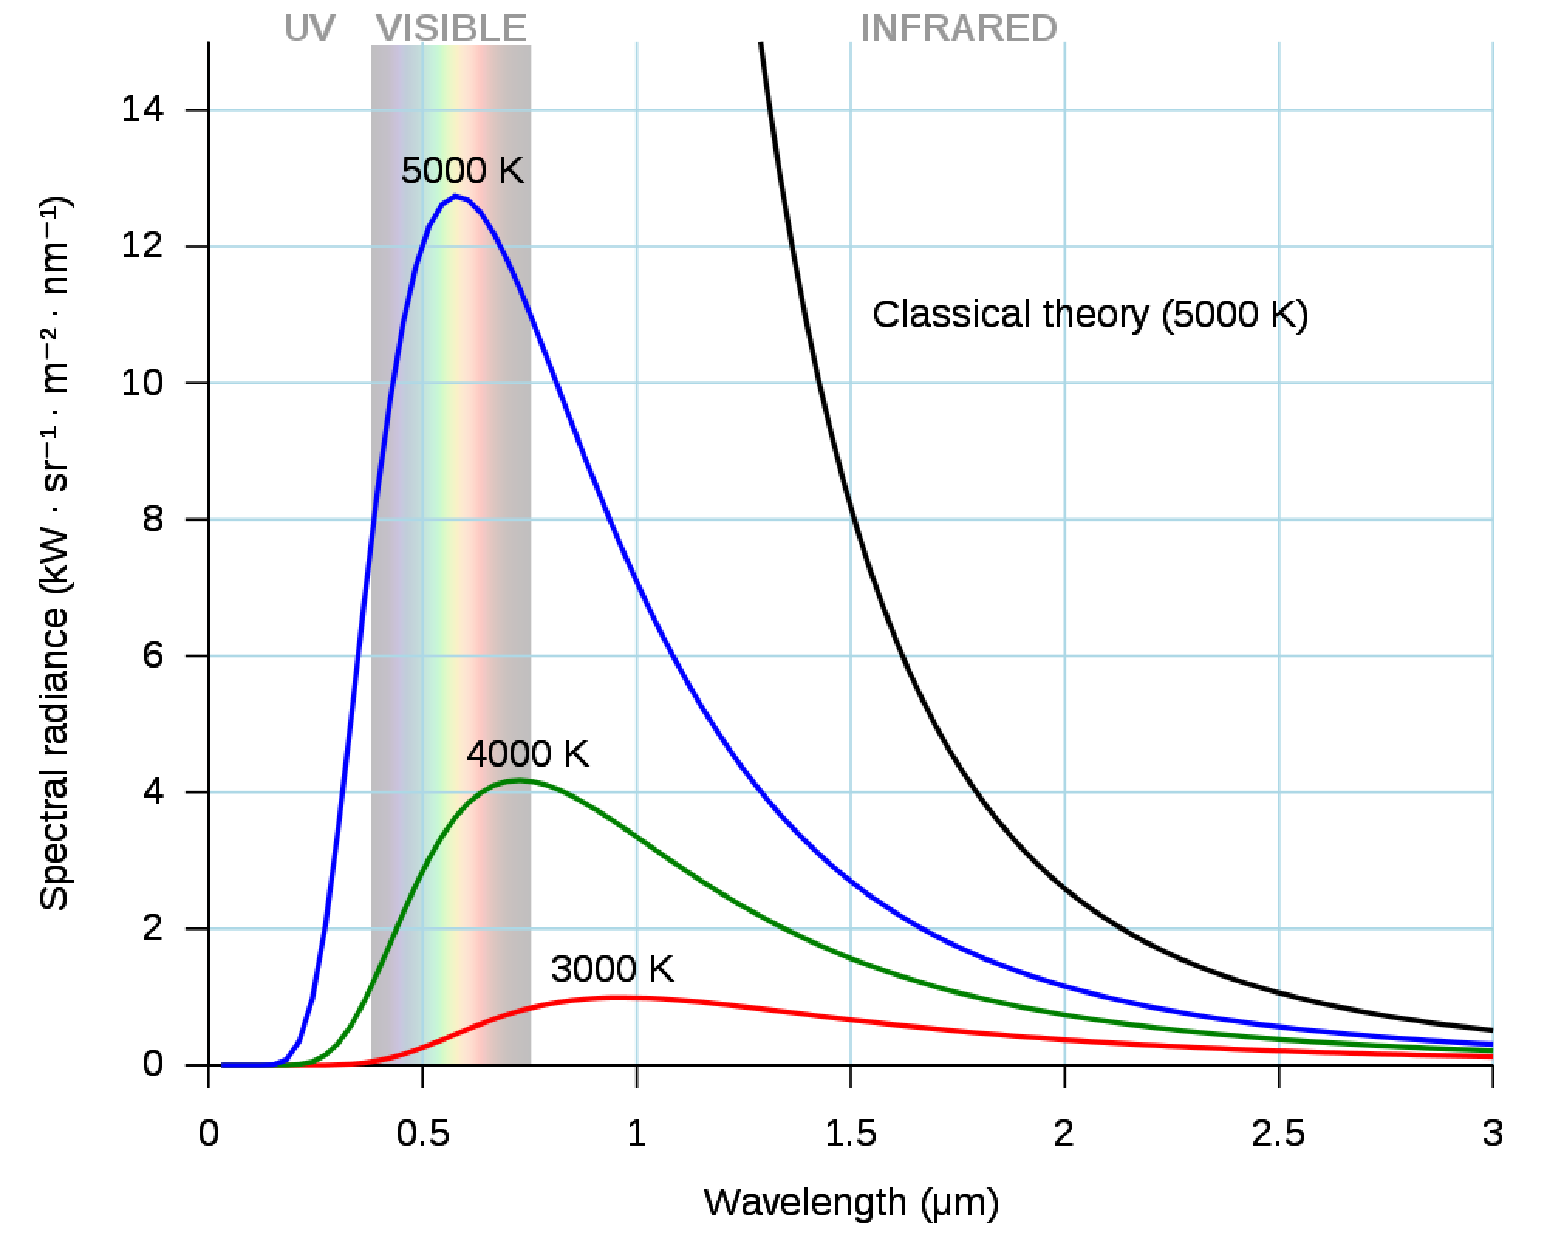
\includegraphics[width=\textwidth]{figs/week08_spectrum.pdf}\end{center}

In this plot the horizontal axis uses the wavelength $\la = 2\pi c / \om$.
Changing variables in your work above, what is Planck spectrum $P(\la)$ as a function of wavelength?
\begin{mdframed}
  $\displaystyle \frac{\vev{E}_{\text{ph}}}{V} = \frac{\hbar}{c^3 \pi^2} \int_0^{\infty} \frac{\om^3}{e^{\be \hbar \om} - 1} \; d\om = $ \\[120 pt] % WARNING: FORMATTING BY HAND
\end{mdframed}

You should find
\begin{equation}
  \label{eq:Planck_la}
  P(\la) = \left(\frac{16\pi^2 \hbar c}{\la^5}\right) \frac{1}{e^{2\pi\be \hbar c / \la} - 1},
\end{equation}
which is plotted\footnote{The plot divides our $P(\la)$ by $4\pi$~steradian and multiplies it by $c$ to convert from an energy density to a spectral power per unit area per unit of solid angle.  For our purposes only the functional form is significant.} for three temperatures $T = 1 / \be$ in the figure above.
Considering first the high-energy ultraviolet (UV) limit of small wavelengths $\la$, we can see from \eq{eq:Planck_la} that $P(\la)$ is exponentially suppressed, which overwhelms the diverging factor $\propto 1 / \la^5$ in parentheses.

In the low-energy infrared limit, the large $\la$ has the same effect that a large temperature ($\be \ll 1$) would have: $e^{2\pi\be \hbar c / \la} - 1 \approx 2\pi\be \hbar c / \la$ and
\begin{equation*}
  P(\la) \approx \left(\frac{16\pi^2 \hbar c}{\la^5}\right) \frac{\la}{2\pi\be \hbar c} = \frac{8\pi T}{\la^4}.
\end{equation*}
The connection to large temperatures indicates that this is what classical statistics would predict for the energy spectrum of light.
It is known as the Rayleigh--Jeans spectrum, named after \href{https://en.wikipedia.org/wiki/John_William_Strutt,_3rd_Baron_Rayleigh}{the third Baron Rayleigh} and \href{https://en.wikipedia.org/wiki/James_Jeans}{James Jeans}.
Recall that the classical approach sums over all possible energies for each degree of freedom, corresponding to a light-emitting object (historically known as a \textit{black body}) emitting light of all wavelengths $\la$.
According to the classical Rayleigh--Jeans spectrum, in the limit $\la \to 0$ this light would carry an infinite amount of energy, an obvious error that became known as the \textit{ultraviolet catastrophe}.
Planck's (heuristic) solution to this conundrum in 1900 was one of the first steps towards the quantum physics that introduces the exponential suppression we computed above.

One final observation we will make about the Planck spectrum shown above is that as the temperature increases, the maximum of the Planck spectrum moves to shorter wavelengths and correspondingly larger energies.
The fact that the peak of the spectrum for $T \approx 5000$~K falls within the wavelengths of visible light (roughly $400$--$700$~nm) is not a coincidence.
As shown in the figure below (from \href{https://commons.wikimedia.org/wiki/File:Solar_Spectrum.png}{Wikimedia Commons}), the amount of sunlight that reaches the surface of the earth is also maximized around visible wavelengths, which are visible to us because we have evolved to make the most efficient use of this sunlight.

Taking into account the absorption of some sunlight by molecules in the atmosphere, we can see from the figure below that the energy spectrum of the sunlight reaching the top of the atmosphere is quite close to a Planck (or `blackbody') spectrum with temperature $T \approx 5778$~K.
The agreement isn't perfect, which is to be expected since the Planck spectrum relies on the non-trivial assumption of an ideal gas of non-interacting particles.
Even with that caveat, numerically fitting the measured sunlight to the Planck spectrum is how the surface temperature of the sun is determined to be $T \approx 5778$~K.
This same fitting procedure can even be done for distant stars, with red stars corresponding to relatively low temperatures $T \lesssim 3500$~K and blue stars corresponding to relatively high temperatures $T \gtrsim 10{,}000$~K.

\begin{center}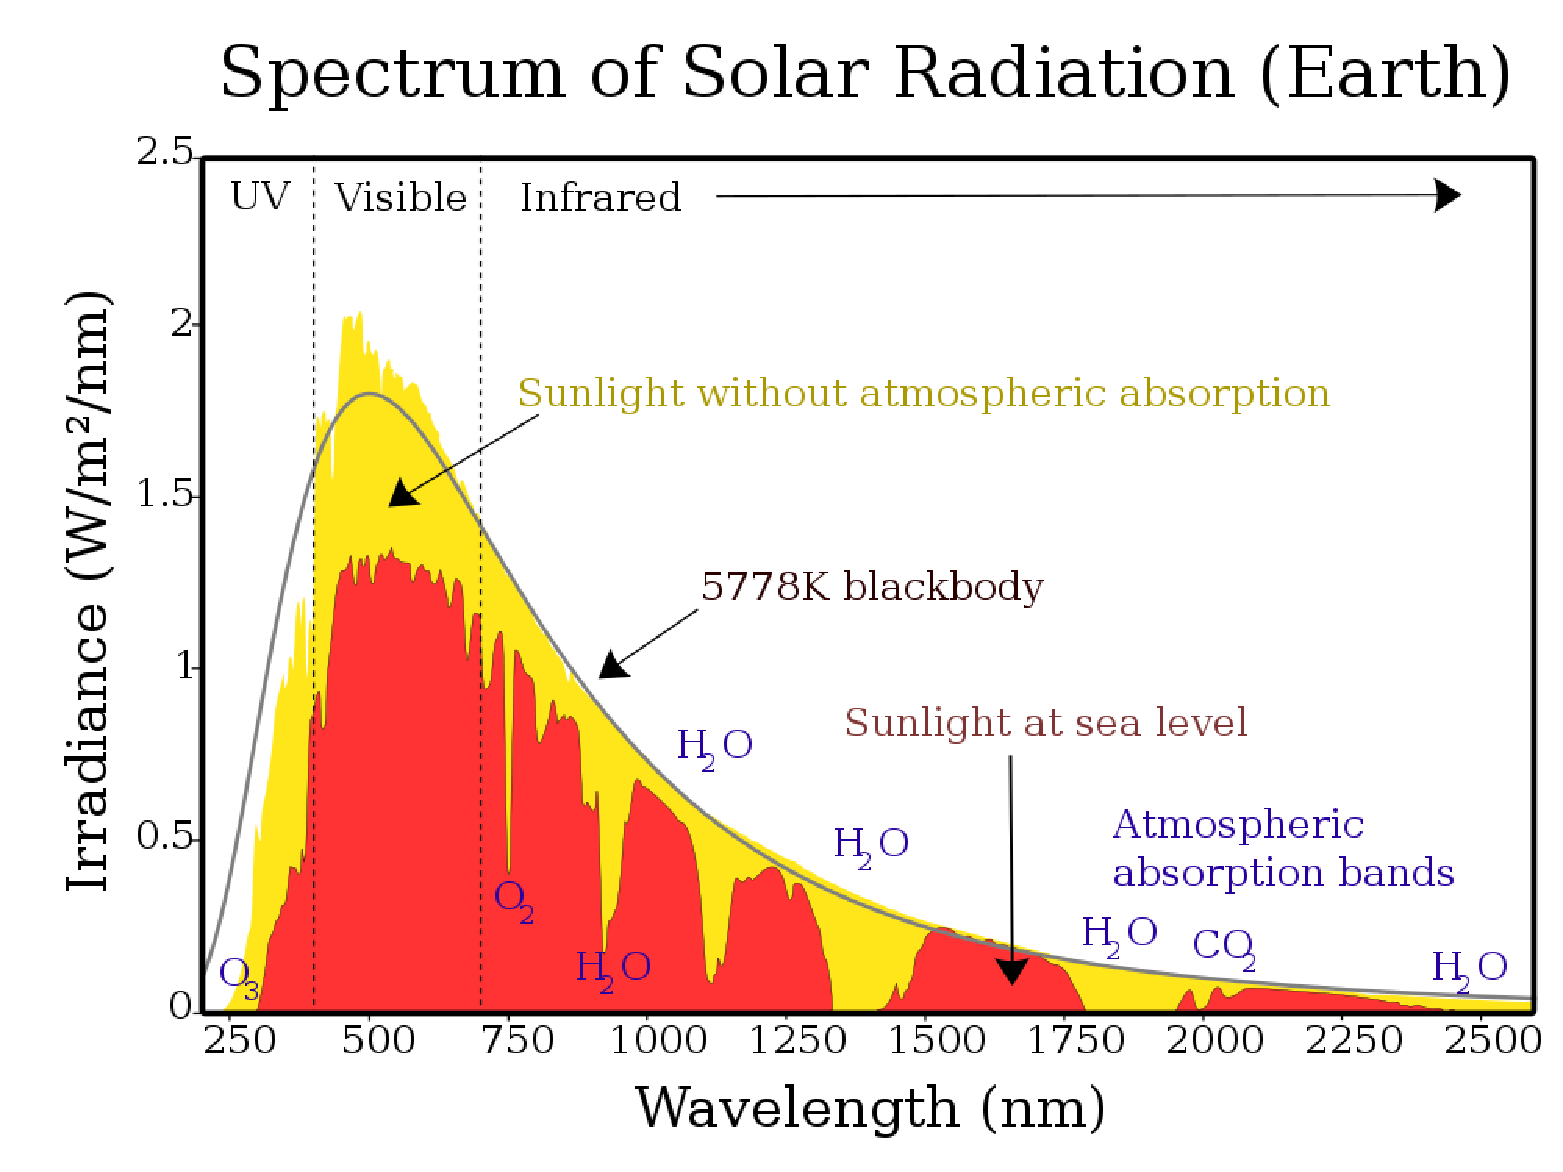
\includegraphics[width=\textwidth]{figs/week08_sun.pdf}\end{center}

In fact, we can even use the Planck spectrum to determine the temperature of inter-galactic space.
Rather than being empty, these voids are actually permeated by a very low-temperature photon gas left over from the Big Bang roughly $14$~billion years ago.
This photon gas is known as the \href{https://en.wikipedia.org/wiki/Cosmic_microwave_background}{cosmic microwave background} (CMB), and carries information about the early evolution of the universe, including some of the strongest evidence for the existence of dark matter.

The picture below is a famous visualization of the CMB, provided by the \href{http://www.esa.int/ESA_Multimedia/Images/2013/03/Planck_CMB}{European Space Agency} and produced from measurements taken by their `Planck' satellite. % Can compare with WMAP from wmap.gsfc.nasa.gov/media/101080/
To produce this image, for each point in the sky the satellite measures the photon spectrum reaching it from that direction.
The contributions coming from stars and galaxies are subtracted, and the remaining data is fit to the Planck spectrum to find the temperature of the intergalactic CMB photon gas at that point.
From point to point, there are only small temperature fluctuations around the average $T_{\text{CMB}} \approx 2.725$~K.
That average temperature is subtracted and the fluctuations themselves are shown below, with warmer red-coloured regions only $\De T \approx 0.0002$~K hotter than the cooler blue-coloured regions.

\begin{center}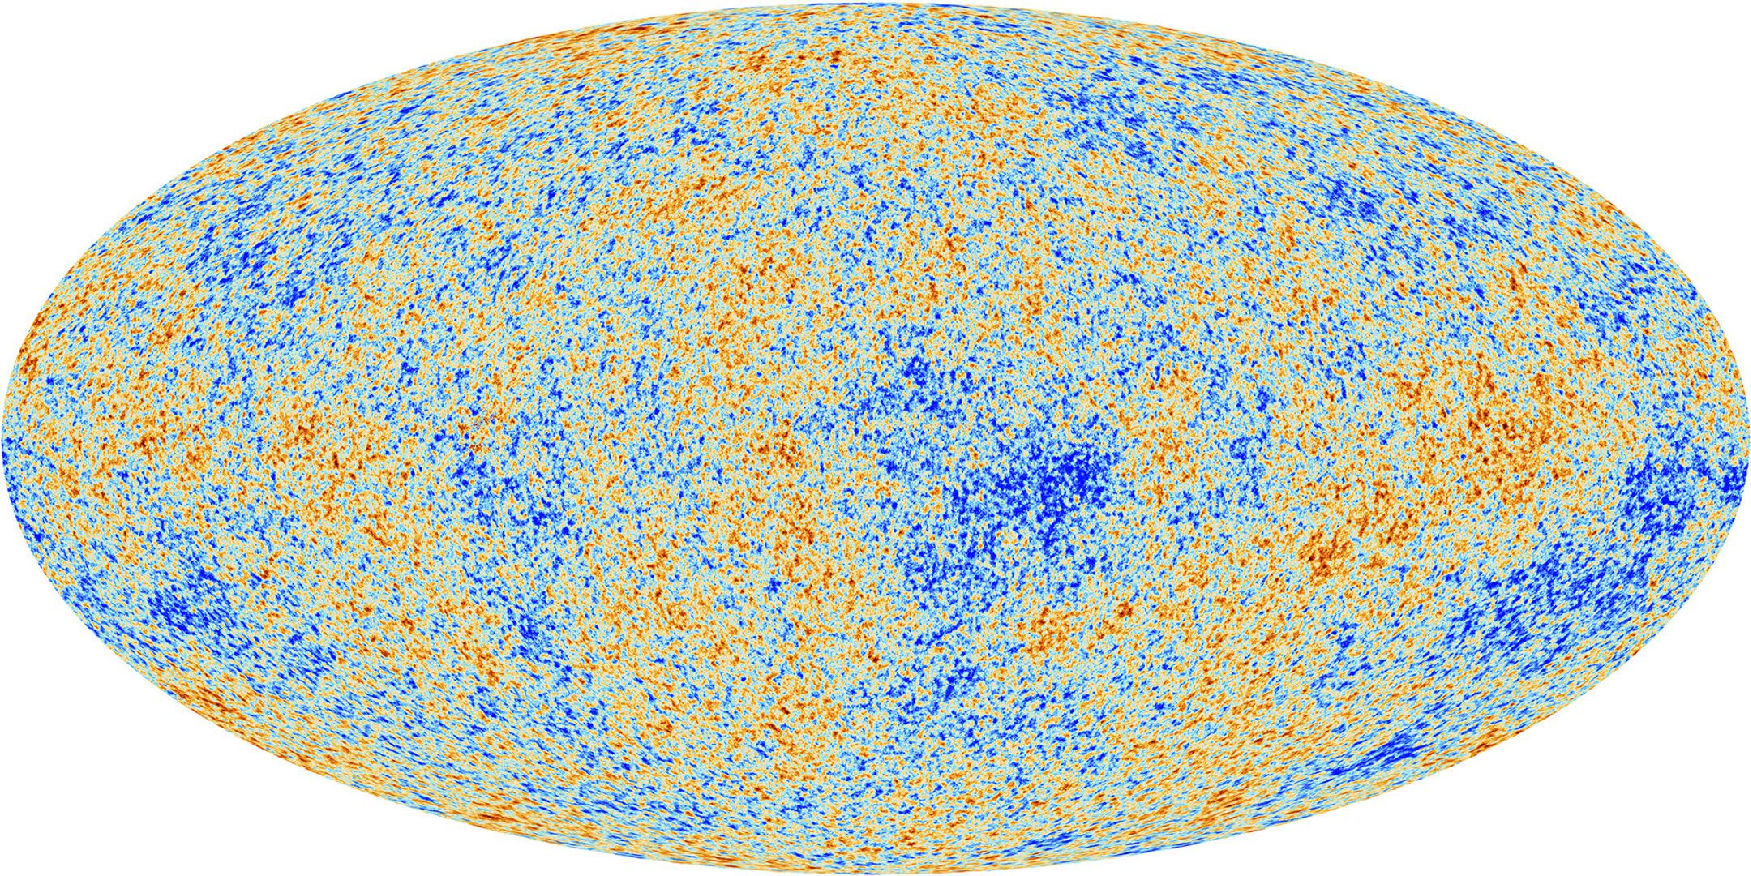
\includegraphics[width=\textwidth]{figs/week08_CMB.pdf}\end{center}

The final figure below illustrates such a fit of CMB data to the Planck spectrum, using measurements taken by the Cosmic Background Explorer (COBE) satellite and \href{https://doi.org/10.1086/185717}{published in 1990}.
(This version of the figure is adapted from that publication, and copied from Schroeder's \textit{Introduction to Thermal Physics}.)
The squares are the measured data, and their size represents a cautious estimate of uncertainties.
They are plotted with the frequency $f = \om / (2\pi)$ on the horizontal axis, with $f \approx 3\cdot 10^{-11}~\text{s}^{-1}$ corresponding to a low-energy wavelength $\la = c / f \approx 1$~mm, roughly $1000$ times longer than the wavelengths of visible light.
The solid line is a fit to the data that produces $T_{\text{CMB}} = 2.735 \pm 0.060$~K.
While more recent satellites have increased the precision with which we know $T_{\text{CMB}}$, this first result was awarded the 2006 Nobel Prize in Physics.

\begin{center}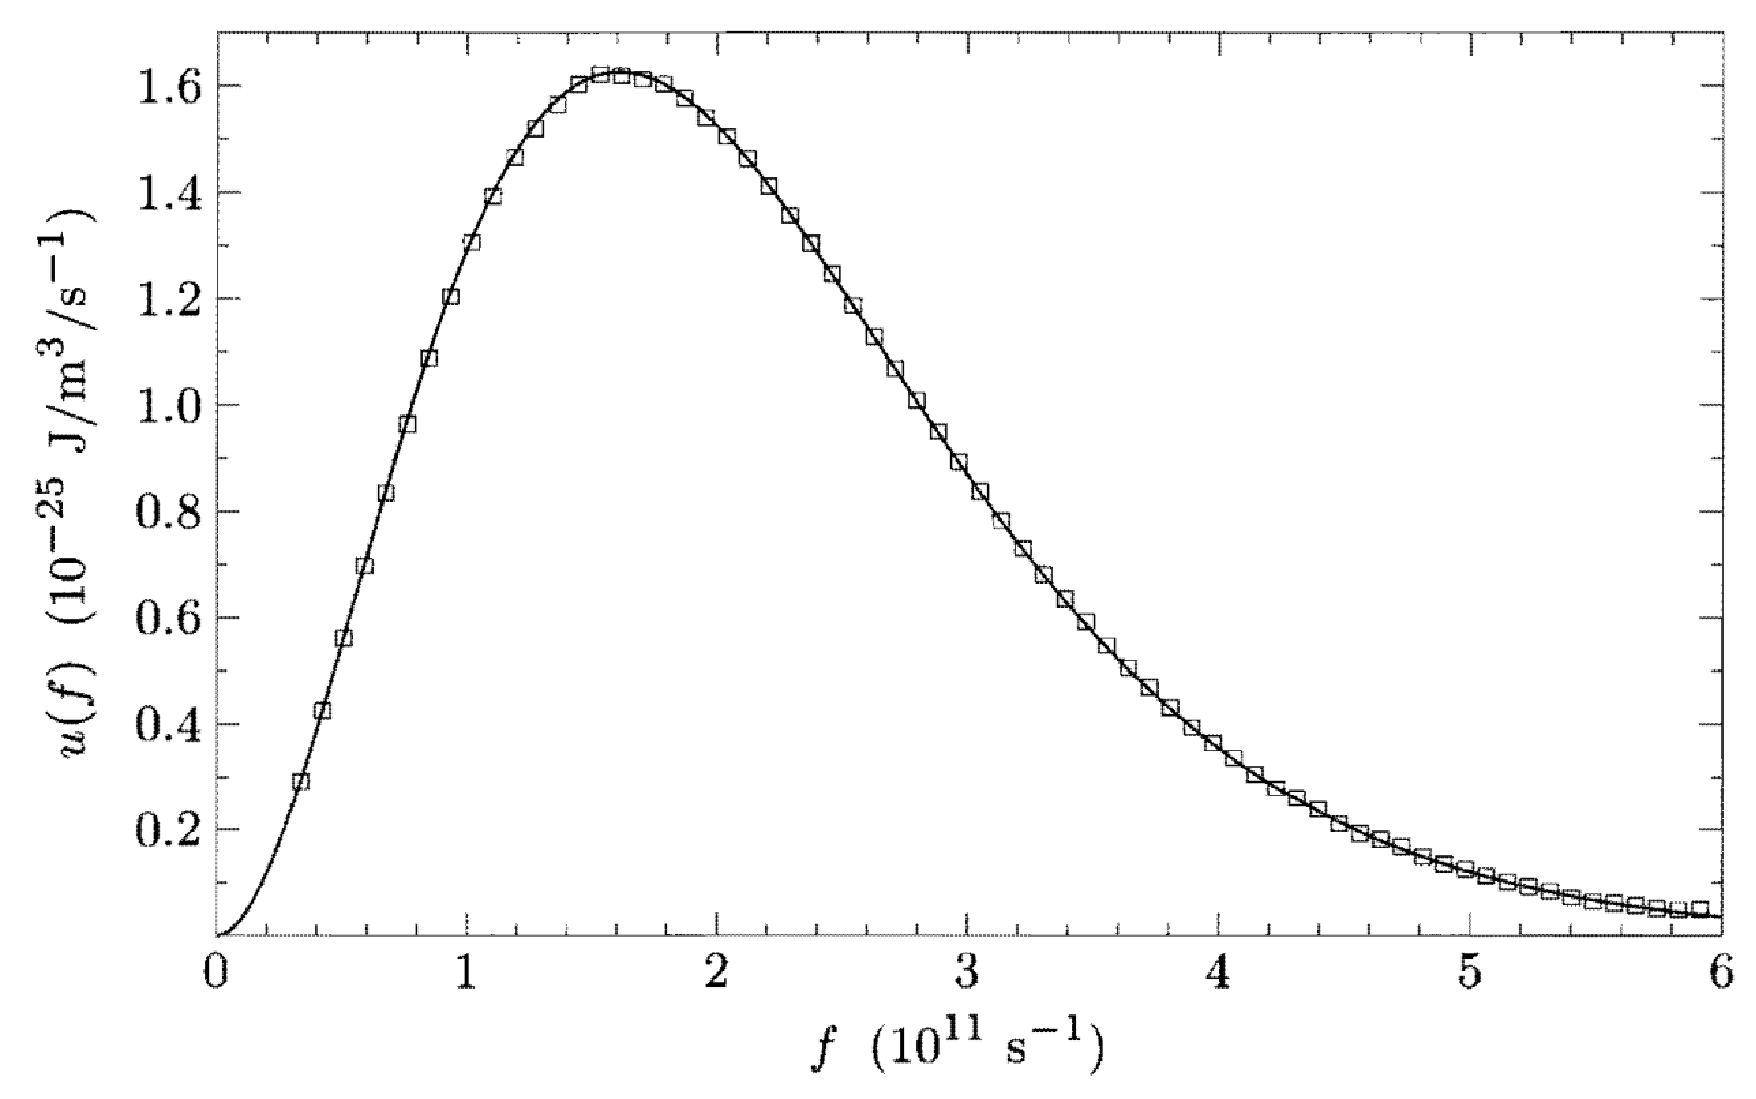
\includegraphics[width=\textwidth]{figs/week08_COBE.pdf}\end{center}

\begin{shaded}
  Even though we derived the Planck spectrum by assuming an ideal gas of non-interacting photons, we see that it provides an excellent mathematical model for real physical systems, stretching from the hottest to the coldest places in the universe.
\end{shaded}
% ------------------------------------------------------------------



% ------------------------------------------------------------------
\subsection{Equation of state for the photon gas}
Having looked in some detail at the integrand for the photon gas energy density, \eq{eq:Planck_omega}, let's complete the integration, which involves a famous integral related to the Riemann zeta function:
\begin{equation*}
  I_4 = \int_0^{\infty} \frac{x^3}{e^x - 1} dx = \Gamma(4) \zeta(4) = \frac{\pi^4}{15}.
\end{equation*}
Using this result, what is the ideal photon gas energy density?
\begin{mdframed}
  $\displaystyle \frac{\vev{E}_{\text{ph}}}{V} = \frac{\hbar}{c^3 \pi^2} \int_0^{\infty} \frac{\om^3}{e^{\be \hbar \om} - 1} \; d\om = $ \\[100 pt]
\end{mdframed}

You should find a result proportional to $T^4$.
It would be ideal (sorry) if we could put this in a form as simple as \eq{eq:ideal_energy} for the energy of an $N$-particle non-relativistic ideal gas in the canonical ensemble.
Now that we are working in the grand-canonical ensemble, this requires computing the average photon number from \eq{eq:N_grand},
\begin{equation*}
  \vev{N}_{\text{ph}} = -\left. \pderiv{}{\mu} \Phi_{\text{ph}}\right|_{\mu = 0} = -\left. \frac{VT}{c^3 \pi^2} \int_0^{\infty} d\om \; \om^2 \pderiv{}{\mu} \log\left[1 - e^{-\be \hbar \om} e^{\be \mu}\right] \right|_{\mu = 0}.
\end{equation*}
recalling $\mu = 0$ for photon gases.
The calculation is quite similar to that for the average internal energy density, now involving the integral
\begin{equation*}
  I_3 = \int_0^{\infty} \frac{x^2}{e^x - 1} dx = \Gamma(3) \zeta(3) = 2\zeta(3).
\end{equation*}
\newpage % WARNING: FORMATTING BY HAND
\noindent Using this result, what is the ideal photon gas number density?
\begin{mdframed}
  $\displaystyle \frac{\vev{N}_{\text{ph}}}{V} = \frac{1}{c^3 \pi^2} \int_0^{\infty} \frac{\om^2}{e^{\be \hbar \om} - 1} \; d\om = $ \\[100 pt]
\end{mdframed}

You should find a result proportional to $T^3 \propto \vev{E}_{\text{ph}} / T$, so that
\begin{equation}
  \vev{E}_{\text{ph}} = \frac{\pi^2}{15 \hbar^3 c^3} VT^4 = \frac{\pi^4}{30\zeta(3)} \vev{N}_{\text{ph}} T.
\end{equation}
The functional form is the same as \eq{eq:ideal_energy}, with a larger numerical factor
\begin{equation*}
  \frac{\pi^4}{30\zeta(3)} = \frac{\Gamma(4) \zeta(4)}{\Gamma(3) \zeta(3)} \approx 2.7
\end{equation*}
compared to the $\frac{3}{2}$ for the classical non-relativistic case.

To get the rest of the way to the equation of state for the photon gas, we need to compute the \textit{radiation pressure}
\begin{equation*}
  P_{\text{ph}} = -\left. \pderiv{}{V} \vev{E}_{\text{ph}} \right|_{S_{\text{ph}}},
\end{equation*}
which requires first figuring out the condition of constant entropy $S_{\text{ph}}$ for a photon gas.
From \eq{eq:grand_relation} with $\mu = 0$, we have
\begin{equation*}
  S_{\text{ph}} = \frac{\vev{E}_{\text{ph}} - \Phi_{\text{ph}}}{T}.
\end{equation*}
Looking back to \eq{eq:photon_grand} for the grand-canonical potential, we see
\begin{equation*}
  \frac{\Phi_{\text{ph}}}{T} = \frac{V}{c^3 \pi^2} \int_0^{\infty} d\om \; \om^2 \log\left[1 - e^{-\be \hbar \om}\right] = \frac{VT^3}{\hbar^3 c^3 \pi^2} \int_0^{\infty} dx \; x^2 \log\left[1 - e^{-x}\right],
\end{equation*}
changing variables to $x = \be \hbar \om = \hbar \om / T$.
The final factor in this expression is yet another delightful integral,
\begin{equation*}
  \int_0^{\infty} dx \; x^2 \log\left[1 - e^{-x}\right] = -2\zeta(4) = -\frac{\pi^4}{45}.
\end{equation*}
Since this gives us $S \propto VT^3$, we can conclude that the condition of constant entropy for a photon gas is $V T^3 = \mbox{constant}$, in contrast to the $V T^{3/2}$ dependence of \eq{eq:ideal_entropy} for classical non-relativistic particles.

\newpage % WARNING: FORMATTING BY HAND
At this point we just need to insert the constant-entropy condition $T = b V^{-1 / 3}$ (with $b$ a constant) into the average internal energy and take the derivative:
\begin{mdframed}
  $\displaystyle P = -\left. \pderiv{}{V} \vev{E}_{\text{ph}} \right|_{S_{\text{ph}}} = -\pderiv{}{V} \frac{\pi^2}{15 \hbar^3 c^3} b^4 V^{-1 / 3} = $ \\[100 pt]
\end{mdframed}
You should find the following equation of state for the photon gas,
\begin{equation}
  P_{\text{ph}} V = \frac{1}{3} \vev{E}_{\text{ph}} = \frac{\pi^4}{90\zeta(3)} \vev{N}_{\text{ph}} T.
\end{equation}
The functional form is the same as the (classical, non-relativistic) ideal gas law, with just an additional numerical factor
\begin{equation*}
  \frac{\pi^4}{90\zeta(3)} = \frac{\zeta(4)}{\zeta(3)}.
\end{equation*}
% ------------------------------------------------------------------
